\documentclass[a4paper,14pt]{article}
\usepackage{float}
\usepackage{extsizes}
\usepackage{amsmath}
\usepackage{amssymb}
\everymath{\displaystyle}
\usepackage{geometry}
\usepackage{fancyhdr}
\usepackage{multicol}
\usepackage{graphicx}
\usepackage[brazil]{babel}
\usepackage[shortlabels]{enumitem}
\usepackage{cancel}
\columnsep=2cm
\hoffset=0cm
\textwidth=8cm
\setlength{\columnseprule}{.1pt}
\setlength{\columnsep}{2cm}
\renewcommand{\headrulewidth}{0pt}
\geometry{top=1in, bottom=1in, left=0.7in, right=0.5in}

\pagestyle{fancy}
\fancyhf{}
\fancyfoot[C]{\thepage}

\begin{document}
	
	\noindent\textbf{6FMA47~Matemática} 
	
	\begin{center}Cubos (Versão estudante)
	\end{center}
	
	\noindent\textbf{Nome:} \underline{\hspace{10cm}}
	\noindent\textbf{Data:} \underline{\hspace{4cm}}
	
	%\section*{Questões de Matemática}
	
	
    \begin{multicols}{2}
    	Cubos são blocos retangulares com as três dimensões iguais, ou seja, o comprimento a largura e a altura têm a mesma medida. Assim como qualquer bloco retangular, o cubo tem 6 faces, 8 vértices e 12 arestas. Todas as faces de um cubo são quadradas.\\
    	\textsubscript{---------------------------------------------------------------------}
    	\begin{enumerate}
    		\item Com oito cubos iguais podemos construir um cubo maior. Se a medida das arestas dos cubos menores é 8 cm, qual é a medida da aresta do cubo maior construído com os cubos menores?
\\\\\\\\\\\\
    		\item Quantos cubos existem na pilha abaixo? \\
    		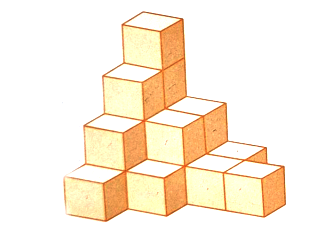
\includegraphics[width=1\linewidth]{6FMA47_imagens/imagem1}
    		~
\\\\
            \item Calcule a soma das medidas de todas as arestas de um cubo cuja aresta mede 6 cm. \\\\\\\\
            \item Doze cubos de 1 cm de aresta são colocados juntos, formando o paralelepípedo representado abaixo. \\ 
            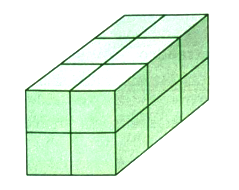
\includegraphics[width=1\linewidth]{6FMA47_imagens/imagem2}
            A superfície do mesmo foi pintada de verde e, em seguida, os cubos foram separados.
            \begin{enumerate}[a)]
            	\item Quantos cubos ficaram com apenas duas faces verdes? \\\\\\\\
            	\item Quantos ficaram com três faces verdes? \\\\
        	\end{enumerate}
            \item Dado um cubo de 2 cm de lado e outro com 1 cm de lado você pode observar que é possível colocar $8=2^3$ cubos menores dentro do cubo maior, conforme a figura. Um fabricante de refrigerantes vende sua bebida em duas embalagens. A primeira é uma garrafa de 30 cm de altura e a segunda é uma miniatura da primeira, com altura de 15 cm. Usando a mesma ideia dos cubos e sabendo que o volume da garrafa maior é 2.000 ml, calcule o volume da garrafa menor.
            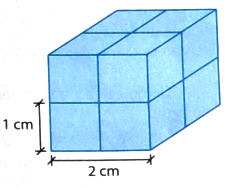
\includegraphics[width=1\linewidth]{6FMA47_imagens/imagem3}
            
        \end{enumerate}    
    $~$ \\ $~$ \\ $~$ \\ $~$ \\ $~$ \\ $~$ \\ $~$ \\ $~$ \\ $~$ \\ $~$ \\ $~$ \\ $~$ \\ $~$ \\ $~$ \\ $~$ \\ $~$ \\ $~$ \\ $~$ \\ $~$ \\ $~$ \\ $~$ \\ $~$ \\ $~$ \\ $~$ \\ $~$ \\ $~$ \\ $~$ \\ $~$ \\ $~$ \\ $~$ \\ $~$ \\ $~$ \\ $~$ \\ $~$ \\ $~$ \\ $~$ \\ $~$ \\ $~$ \\ $~$ \\ $~$ \\ $~$ \\ $~$ \\ $~$ \\ $~$ \\ $~$ \\ $~$ \\ $~$ \\ $~$ \\ $~$ \\ $~$ \\ $~$ \\ $~$ \\ $~$ \\ $~$ \\ $~$ \\ $~$ \\ $~$ \\
    \end{multicols}
\end{document}